\documentclass[journal]{IEEEtran}
\usepackage{graphicx}
\graphicspath{ {../report/} }
\usepackage{hyperref}

\ifCLASSINFOpdf
\else
\fi

\hyphenation{op-tical net-works semi-conduc-tor}

\begin{document}


\title{GPU Optimized Pedestrian Detection}


\author{Sam Kreter}

\markboth{High Performance Computing}
{Shell \MakeLowercase{\textit{et al.}}: Bare Demo of IEEEtran.cls for IEEE Journals}

\maketitle

\begin{abstract}
The OpenCV library has a good CPU and GPU implementation of a Histogram of Oriented Gradients as well as an Support Vector Machine. This paper will go through the comparisons of the two implementations for finding and identify objects on different size images. It will also look into the effect that the number of threads per block has on the final computation time of the GPU implementation.
\end{abstract}

\begin{IEEEkeywords}
    HOG (Histogram of Oriented Gradients), SVM (Support Vector Machine), OpenCV, GPU, Cuda
\end{IEEEkeywords}

\IEEEpeerreviewmaketitle

\section{Introduction}
\IEEEPARstart{P}{edestrian} detection is a main component in many applications such as crowd control systems and people tracking. One common way of implementing a people detection system is using a Histogram of Oriented Gradients to extract the features from an image and an Support Vector Machine to classify each element of the image as a person or not. HOG works by segmenting the image in many windows then creating a histogram of the orientations or directions of each cell of the segment. The histograms are then concatenated together to create a feature vector of floating points. The SVM then takes the feature vector to classify the objects found in the image. \\

\section{Implementation}
    In order to implement the Pedestrian detection system, it is necessary to have an implementation of a Histogram of Oriented Gradients and a SVM that is trained on the HOG features of a person in different walking positions. The openCV library comes with both a standard CPU implementation and a accelerated GPU implementation of both the HOG feature extraction as well as the pre trained SVM. \\

\subsection{CPU Implementation}

    For OpenCV’s CPU implementation, the HOG feature extractor is abstracted into an object where simple function calls are used to set the different properties and load the image. The object itself comes with a built in function “getDefaultPeopleDetector()” that will return OpenCV’s pre trained SVM which then is passed into a simple “setSVMDetector()” to set the SVM for the object. Then with one call to a detectMultiScale function the openCV will compute the HOG for the image and return the specifications such as the location width and height for the detected objects.
    From an interface perspective the GPU implementation works almost the same as the CPU implementations. It is abstracted into an object but instead of instantiating the object, a function call will return a pointer to it. The rest of the implementation follows the CPU except for before the detection is a function call to “upload” the image to the GPU which is an abstraction for the cudamemcpy. \\

\subsection{GPU Implementation}

    The GPU implementation under the hood make use of three kernel functions that run on the GPU, one to compute the gradients, one to compute the histogram and one to classify the histogram. Due to the abstraction that OpenCV uses around the Cuda code for the GPU kernels, it was necessary to build the OpenCV library from source and recompile the code base with changes to the number of threads per block passed to the kernel on the GPU.
    The library’s original code had 256 hard coded in for the number of threads per block in the  compute gradients and classify histogram kernels. The compute histogram uses the number of cells in the histogram as a base for the number of threads per block. \\

    After compiling and installing the modified library I used put together the both the CPU and GPU implementations in order to build the pedestrian Detector.



\section{Experiments}


In order to get quantitative results for the speed up that comes with the GPU, I used a simple image of 4 people walking. I then timed booth the CPU and GPU implementations’ computation times. I ran this 5 times for each image sizes 550x366 , 1100x732 , 2200x1464 , 2750x1830 , 5500x3660  as well as re compiling the OpenCV library for each of the threads per block sizes  1, 32, 128, 256, 512, 1024. I then took the average of the 5 runs for each combinations to get a more stable final results. I found that the GPU had the greatest speed up time of 4 times faster than the CPU for 128 threads per block and an image size of 2750x1830 or  5500x3660. \\

\begin{figure}[h]
\caption{Size of the Image vs the Computation Time. All GPU kernels are being called with 128 threads per block.}
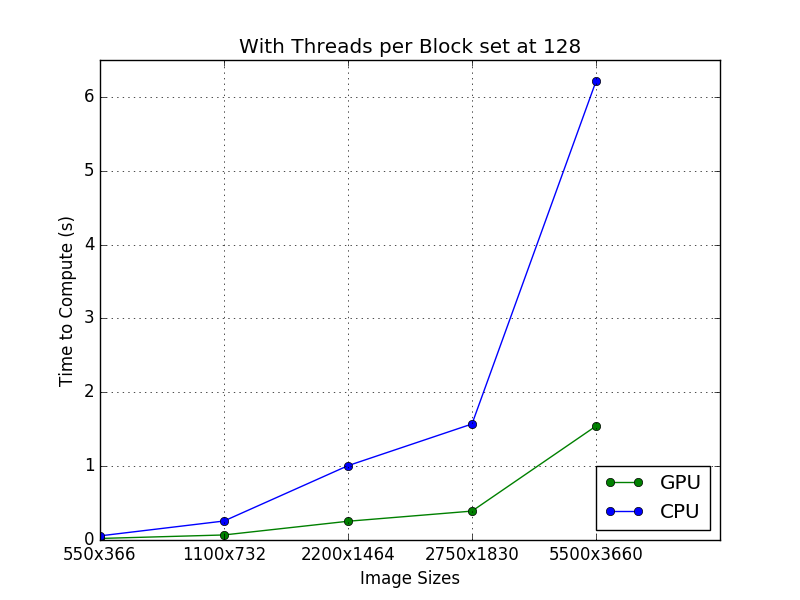
\includegraphics[width=9cm]{SizeTime}
\label{fig:SizeTime}
\end{figure}



Figure \ref{fig:SizeTime} shows the increase speed up of the GPU implementation as the size of the image is increased. The figure also shows that as the image size increases, the CPU implementation’s computation time grows at a much faster rate than the GPU implantation does. \\

\begin{figure}[h]
\caption{Number of threads per block vs the Computation Time. It is hard to tell with the scaling that the gpu times continually decrease until 128 threads per block then slowly increase. Image size of 2750x1830 is used for all tests.}
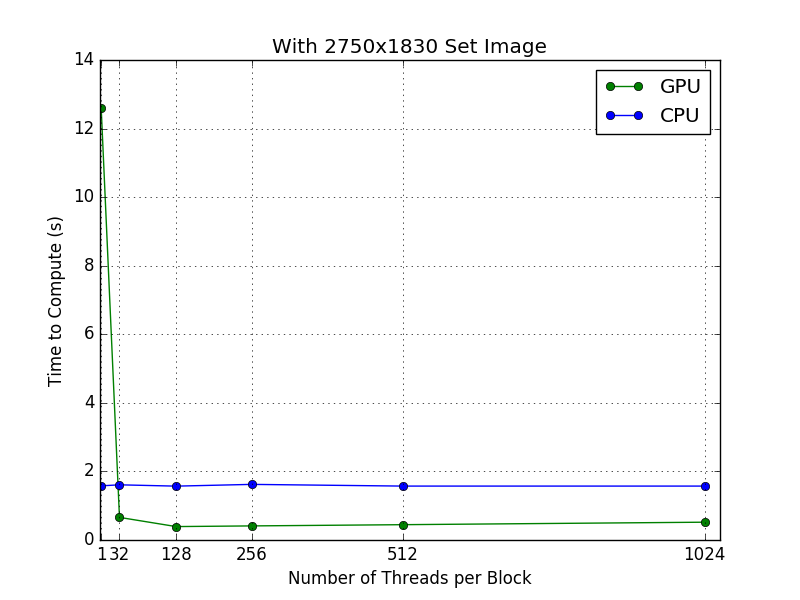
\includegraphics[width=9cm]{ThreadTime}
\label{fig:ThreadTime}
\end{figure}

Figure \ref{fig:ThreadTime} shows that at 1 thread per block the GPU performs much worse than the CPU implementation. This is due to the slow down of having to move the data from the main memory to the GPU’s memory and then the retrieval of the data. After 1 thread per block the GPU takes advantage and hits its maximum speed up at 128 then very slowly starts to have a slower speed up as more threads per block are added. This is due to the overhead of the idle threads per block that do not have work to do on the image.

\section{Challenges}

    One of the biggest challenges I faced was the compilation of the OpenCV library with Cuda capabilities from source. This was not the first time building and installing libraries from source but it turned out to be very challenging to have the correct build flags set to compile for the specific GPU software on the AWS Nvidia AMI that I used for deployment. It took many iterations of rebuilding with different flags and installing dependencies to finally get a working version that could be modified rebuild and reinstalled. \\

    Anther challenge I faced was dealing with the AWS Nvidia AMI. None of the Cuda examples were installed with the SDK. One of the biggest problems I faced with the AMI was that I would repeatedly get an error “(-217) all CUDA-capable devices are busy or unavailable in function allocate” and would have to completely stop the machine then start it in order to have the proper connection with the GPUs. \\

    A final challenge was with the differences between OpenCV 2 and 3’s implementation of Cuda abstraction. In order to make the final program I went through a lot of the source code to find how to use the interfaces for the GPU. \\


\section{Conclusion}
OpenCV shows that for a GPU pedestrian detection system using HOG and the default pre trained SVM should be around 8 times faster than the CPU implementation which can be seen in figure \ref{fig:opencvSpeed}. My final results show that at the fastest point which is using 128 threads per block on and image larger than 2750x1830 I would only have the GPU implementation at 4 times that of the CPU implementation. \\

\begin{figure}[h]
\caption{OpenCV's chart for GPU speed up compared to CPU.}
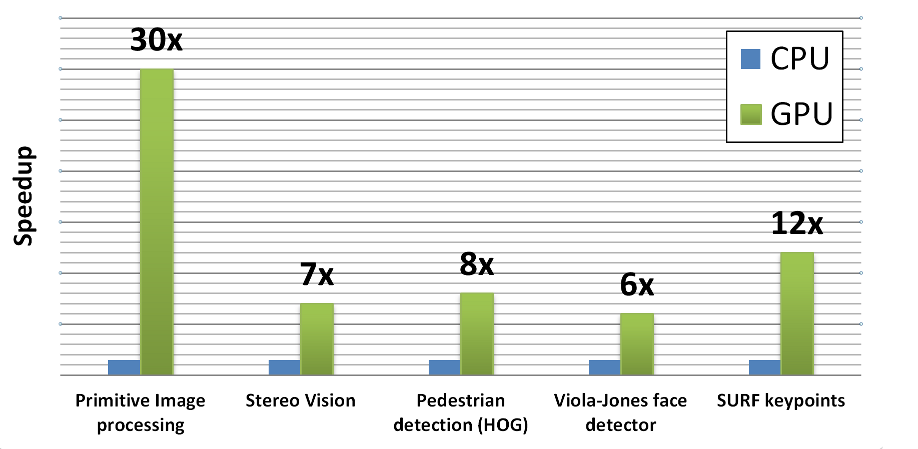
\includegraphics[width=9cm]{opencvSpeed}
\label{fig:opencvSpeed}
\end{figure}


I also found it interesting that after 1 thread per block the number of threads per block had a very small impact on the processing speed of the GPU. One reason for this is that calculating the grid size and number of blocks based off of the threads per block helps eliminate idle threads.



\ifCLASSOPTIONcaptionsoff
  \newpage
\fi

\begin{thebibliography}{1}

\bibitem{OpenCVCuda}
  \emph{OpenCV Cuda Comparison} \url{http://opencv.org/platforms/cuda.html}

\bibitem{OpenCVHog}
  Tulloch, Andrew. \emph{OpenCV Cuda HOG Docs} \url{http://docs.opencv.org/3.0-beta/modules/cuda/doc/object_detection.html}

\end{thebibliography}

\end{document}